\chapter{Architecture}

This chapter explains the architecture of the software in detail. From the very first beginning it was one of the main goals to achive high modularity so that individual parts can be enhanced or replaced easily. The software is seperated into the framework and the application part which in turn consist of multiple modules. Figure \ref{fig:arch} shows the architecture in detail.

\vspace{1cm}

\begin{figure}[h]
\centering
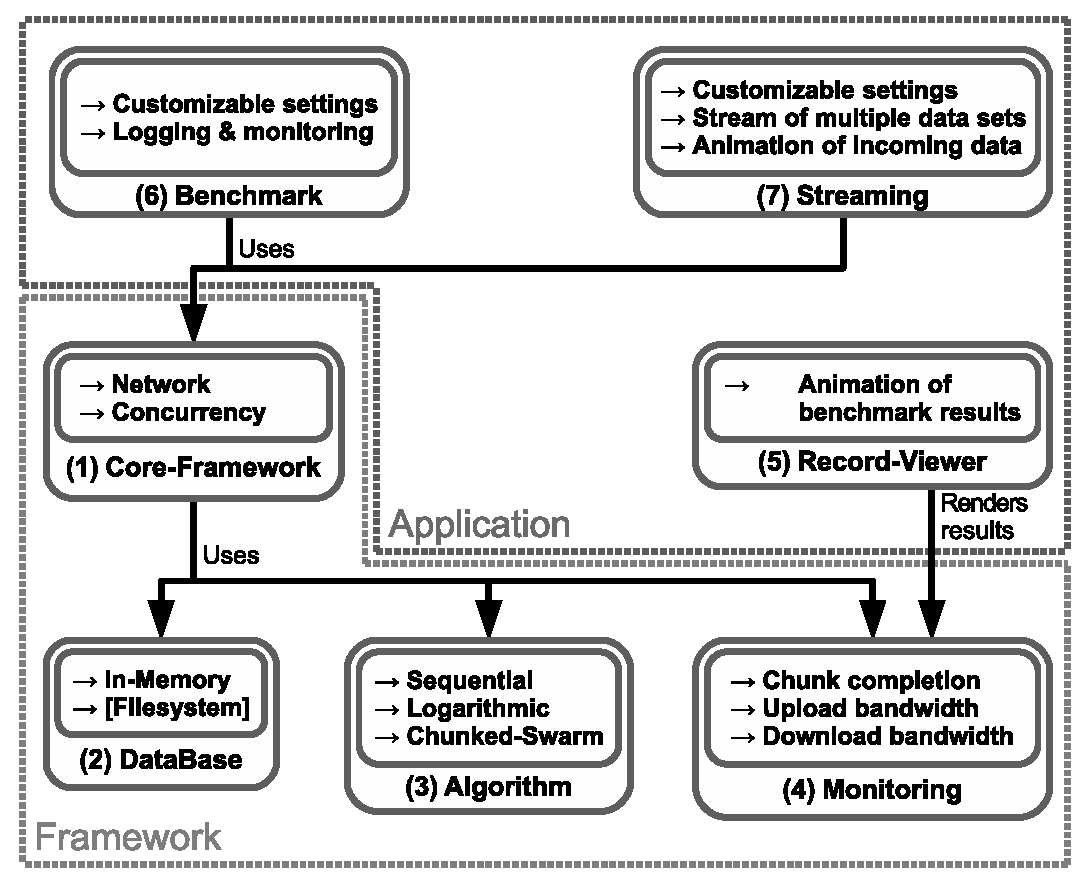
\includegraphics[width=12cm]{arch}
\caption{Software architecture}
\label{fig:arch}
\end{figure}

\clearpage

The application part depends on the Core-Framework and the Monitoring module. It contains three modules which are Benchmark, Streaming and Record-Viewer. The Benchmark module is the most important application part because it can help to create, monitor and evaluate different scenarios in terms of performance and efficiency. All measurements were done using this module. The Streaming module is related to future work and demonstrates the possibility for an incremental stream of data sets. The Record-Viewer module can render and animate results taken from the Monitoring module which is part of the framework part and thus only depends on it.

The framework part contains the Core-Framework, DataBase, Algorithm and Monitoring module. While the DataBase, Algorithm and Monitoring module can be replaced or even omitted the Core-Framework module is the most important module. It manages network, concurrency and the communication of the three other modules located in the framework part. 

The DataBase module represents an interface for a generic data source which might be the filesystem or even completely virtual. This way the framework is able to transfer any kind of data.

The Algorithm module contains the implementations of the concepts presented before which include a sequential, logarithmic and chunked-swarm algorithm. To implement and test new distribution algorithms only this module has to be modified.

The Monitoring module records data like current bandwidth usage and chunk completion which are important data points for evaluating algorithms. This module creates csv files which can be plotted with tools like gnuplot and a log file which contains a chronological stream of events happend during the recording which can be rendered using the Record-Viewer module.
